\documentclass{minimal}

\usepackage{makecell}
\usepackage{tikz}
\usetikzlibrary{arrows,automata}

\begin{document}
\begin{center}
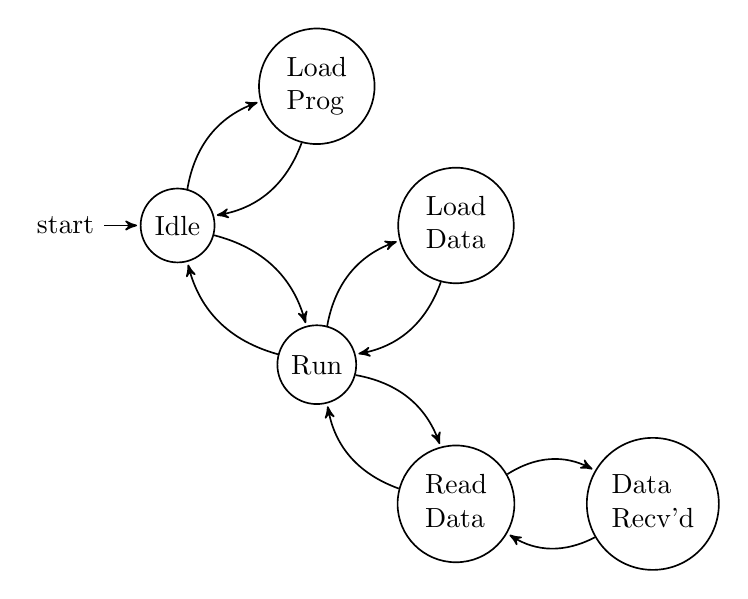
\begin{tikzpicture}[->,>=stealth',shorten >=1pt,auto,node distance=2.5cm,
                    semithick, bend angle=30]
  \tikzstyle{every state}=[fill=none,draw,text=black]
  \node[initial,state] (idle) {Idle};
  \node[state] (load-prog)  [above right of = idle] {\makecell[l]{Load\\Prog}};
  \node[state] (run)        [below right of = idle] {Run};
  \node[state] (load-data)  [above right of = run]  {\makecell[l]{Load\\Data}};
  \node[state] (read-data)  [below right of = run]  {\makecell[l]{Read\\Data}};
  \node[state] (data-recvd) [right of = read-data] {\makecell[l]{Data\\Recv'd}};

  \foreach \a/\b in {idle/load-prog, idle/run, run/load-data, run/read-data,
    read-data/data-recvd} 
    \path[->] (\a) edge [bend left] (\b)
              (\b) edge [bend left] (\a);
\end{tikzpicture}
\end{center}
\end{document}
